\documentclass[11pt,a4paper,twoside,openright]{report}

\usepackage[top=25mm,bottom=25mm,right=25mm,left=30mm,head=12.5mm,foot=12.5mm]{geometry}
\let\openright=\cleardoublepage

\usepackage[a-2u]{pdfx}

\usepackage[
   backend=biber
%  ,style=iso-authoryear
  ,style=alphabetic
  ,citestyle=numeric
  ,sortlocale=cs_CZ
  ,bibencoding=UTF8
  %,block=ragged
]{biblatex}
\addbibresource{references.bib}

%% Přepneme na českou sazbu, fonty Latin Modern a kódování češtiny
\usepackage[czech]{babel}
\usepackage{lmodern}
\usepackage[T1]{fontenc}
\usepackage{textcomp}
\usepackage[utf8]{inputenc}

% Set fonts
\RequirePackage[osf]{mathpazo} % Palatino with oldstyle figures
\newcommand\liningnums[1]{\fontfamily{ppl}\selectfont#1}
\RequirePackage{eulervm}
\RequirePackage[scaled=.8819]{sourcecodepro} % Source Code Pro typeface for monospace

%%% Další užitečné balíčky (jsou součástí běžných distribucí LaTeXu)
\usepackage{amsmath}        % rozšíření pro sazbu matematiky
\usepackage{amsfonts}       % matematické fonty
\usepackage{amsthm}         % sazba vět, definic apod.
\usepackage{bm}             % tučné symboly (příkaz \bm)
\usepackage{graphicx}       % vkládání obrázků
\usepackage{fancyvrb}       % vylepšené prostředí pro strojové písmo
\usepackage{fancyhdr}       % prostředí pohodlnější nastavení hlavy a paty stránek
\usepackage{icomma}         % inteligetní čárka v matematickém módu
\usepackage{dcolumn}        % lepší zarovnání sloupců v tabulkách
\usepackage{booktabs}       % lepší vodorovné linky v tabulkách
\makeatletter
\@ifpackageloaded{xcolor}{
   \@ifpackagewith{xcolor}{usenames}{}{\PassOptionsToPackage{usenames}{xcolor}}
  }{\usepackage[usenames]{xcolor}} % barevná sazba
\makeatother
\usepackage{multicol}       % práce s více sloupci na stránce
\usepackage{caption}
\usepackage{enumitem}
\usepackage{lipsum}
\setlist[itemize]{noitemsep, topsep=0pt, partopsep=0pt}
\setlist[enumerate]{noitemsep, topsep=0pt, partopsep=0pt}
\setlist[description]{noitemsep, topsep=0pt, partopsep=0pt}
\usepackage{pdfpages}

\usepackage{tocloft}
\setlength\cftparskip{0pt}
\setlength\cftbeforechapskip{1.5ex}
\setlength\cftfigindent{0pt}
\setlength\cfttabindent{0pt}
\setlength\cftbeforeloftitleskip{0pt}
\setlength\cftbeforelottitleskip{0pt}
\setlength\cftbeforetoctitleskip{0pt}
\renewcommand{\cftlottitlefont}{\Huge\bfseries}
\renewcommand{\cftloftitlefont}{\Huge\bfseries}
\renewcommand{\cfttoctitlefont}{\Huge\bfseries}

% vyznaceni odstavcu
\parindent=0pt
\parskip=11pt

% zakaz vdov a sirotku - jednoradkovych pocatku ci koncu odstavcu na prechodu mezi strankami
\clubpenalty=1000
\widowpenalty=1000
\displaywidowpenalty=1000

% nastaveni radkovani
\renewcommand{\baselinestretch}{1.20}

% nastavení hlavy a paty stránek
\fancyhf{}
\renewcommand{\chaptermark}[1]{\markboth{#1}{}}
\fancyhead[RO,LE]{\leftmark}
\fancyfoot[RO,LE]{\thepage}
%\renewcommand{\footrulewidth}{0pt}
\fancypagestyle{plain}{%
\fancyhf{} % clear all header and footer fields
\fancyfoot[RO,LE]{\thepage}
\renewcommand{\headrulewidth}{0pt}
%\renewcommand{\footrulewidth}{0.5pt}
}

% Tato makra přesvědčují mírně ošklivým trikem LaTeX, aby hlavičky kapitol
% sázel příčetněji a nevynechával nad nimi spoustu místa. Směle ignorujte.
\makeatletter
\def\@makechapterhead#1{
  {\parindent \z@ \raggedright 
   \Huge\bfseries \thechapter. #1
   \par\nobreak
   \vskip 20\p@
}}
\def\@makeschapterhead#1{
  {\parindent \z@ \raggedright 
   \Huge\bfseries #1
   \par\nobreak
   \vskip 20\p@
}}
\makeatother

% Trochu volnější nastavení dělení slov, než je default.
\lefthyphenmin=2
\righthyphenmin=2

% Zapne černé "slimáky" na koncích řádků, které přetekly, abychom si
% jich lépe všimli.
\overfullrule=1mm

%% Balíček hyperref, kterým jdou vyrábět klikací odkazy v PDF,
%% ale hlavně ho používáme k uložení metadat do PDF (včetně obsahu).
%% Většinu nastavítek přednastaví balíček pdfx.
\hypersetup{unicode}
\hypersetup{breaklinks=true}
\hypersetup{hidelinks}

%%% Prostředí pro sazbu kódu, případně vstupu/výstupu počítačových
%%% programů. (Vyžaduje balíček fancyvrb -- fancy verbatim.)

\DefineVerbatimEnvironment{code}{Verbatim}{fontsize=\small, frame=single}



\def\NazevPrace{Zařízení pro realizaci chytré domácnosti}
\def\Trida{4.C}
\def\AutorPrace{Vladislav Aulich}
\def\DatumOdevzdani{2021}

% Vedoucí práce: Jméno a příjmení s~tituly
\def\Vedouci{Bc. Emil Miler}

% Studijní program a obor
\def\StudijniProgram{studijní program}
\def\StudijniObor{studijní obor}

% Text čestného prohlášení
\def\Prohlaseni{Prohlašuji, že jsem svou práci vypracoval samostatně a použil jsem pouze prameny a literaturu
uvedené v~seznamu bibliografických záznamů. Nemám žádné námitky proti zpřístupňování této práce v~souladu se
zákonem č. 121/2000 Sb. o~právu autorském, o~právech souvisejících s~právem autorským a
o~změně některých zákonů (autorský zákon) ve znění pozdějších předpisů.}

% Text poděkování
\def\Podekovani{%
Touto cestou bych rád poděkoval svému vedoucímu práce Bc. Emilu Milerovi za podporu a odbornou pomoc při tvorbě projektu. Dále bych chěl poděkovat svému bratrovi za pomoc při stavbě 3D tiskárny a odstraňováním následných vad tisku a své sestře za pomoc při testování  a motivaci k dokončení projektu.
}

% Abstrakt česky
\def\Abstrakt{%
Tento projekt se zabývá realizací chytré domácnosti. Pro tvorbu projektu byl zvolen mikrokontrolér Arduino uno a čip ESP32. Komunikace mezi zařízeními je realizovaná bezdrátově za použití otevřené rádiové frekvence 433 MHz. V rámci projektu bylo vytvořeno jednoduché webové rozhraní v HTML. Součástí projektu je i výroba hardware s použitím metody 3D tisku na tiskárně Ender 3 pro. Vývoj kódu probíhal v prostředí Arduino IDE, pro trasování změn byl využit verzovací systém git.
}

% Abstrakt anglicky
\def\AbstraktEN{%
This project deals with the implementation of a smart home. The project is created using an Arduino uno microcontroller and an ESP32. Communication between devices is realized wirelessly using an open radio frequency of 433 MHz. Within the project, a simple web interface in HTML was created. The project also includes the production of hardware using the 3D printing method on the Ender 3 pro printer. The code was developed in the Arduino IDE environment, and the git versioning system was used to trace the changes.
}

% 3 až 5 klíčových slov
\def\KlicovaSlova{Chytrá domácnost, automatizace, ESP32, Arduino, Arduino IDE, 433 MHz, HTML}
% 3 až 5 klíčových slov anglicky
\def\KlicovaSlovaEN{smart home, automation, ESP32, Arduino, Arduino IDE, 433 MHz, HTML}

\begin{document}

%%% Titulní strana práce a další povinné informační strany

%%% Titulní strana práce

\pagestyle{empty}
\pagenumbering{gobble}
\hypersetup{pageanchor=false}

\begin{center}
\LARGE
\textbf{GYMNASIUM JANA KEPLERA}\\
{\large Parléřova 2/118, 169 00 Praha 6}

\vspace{\stretch{3}}


\includegraphics[width=.3\textwidth]{img/logo}

\vspace{\stretch{3}}

{\Huge\bfseries\NazevPrace}

\vspace{8mm}
\mdseries{Maturitní práce}

\vspace{\stretch{8}}
\large
\begin{tabular}{rl}
Autor: & \AutorPrace \\
\noalign{\vspace{2mm}}
Třída: & \Trida\\
\noalign{\vspace{2mm}}
Školní rok: & 2020/2021\\
\noalign{\vspace{2mm}}
Předmět: & Informatika \\
\noalign{\vspace{2mm}}
Vedoucí práce: & \Vedouci \\
\end{tabular}

\vspace{20mm}
Praha, \DatumOdevzdani
\end{center}


\openright

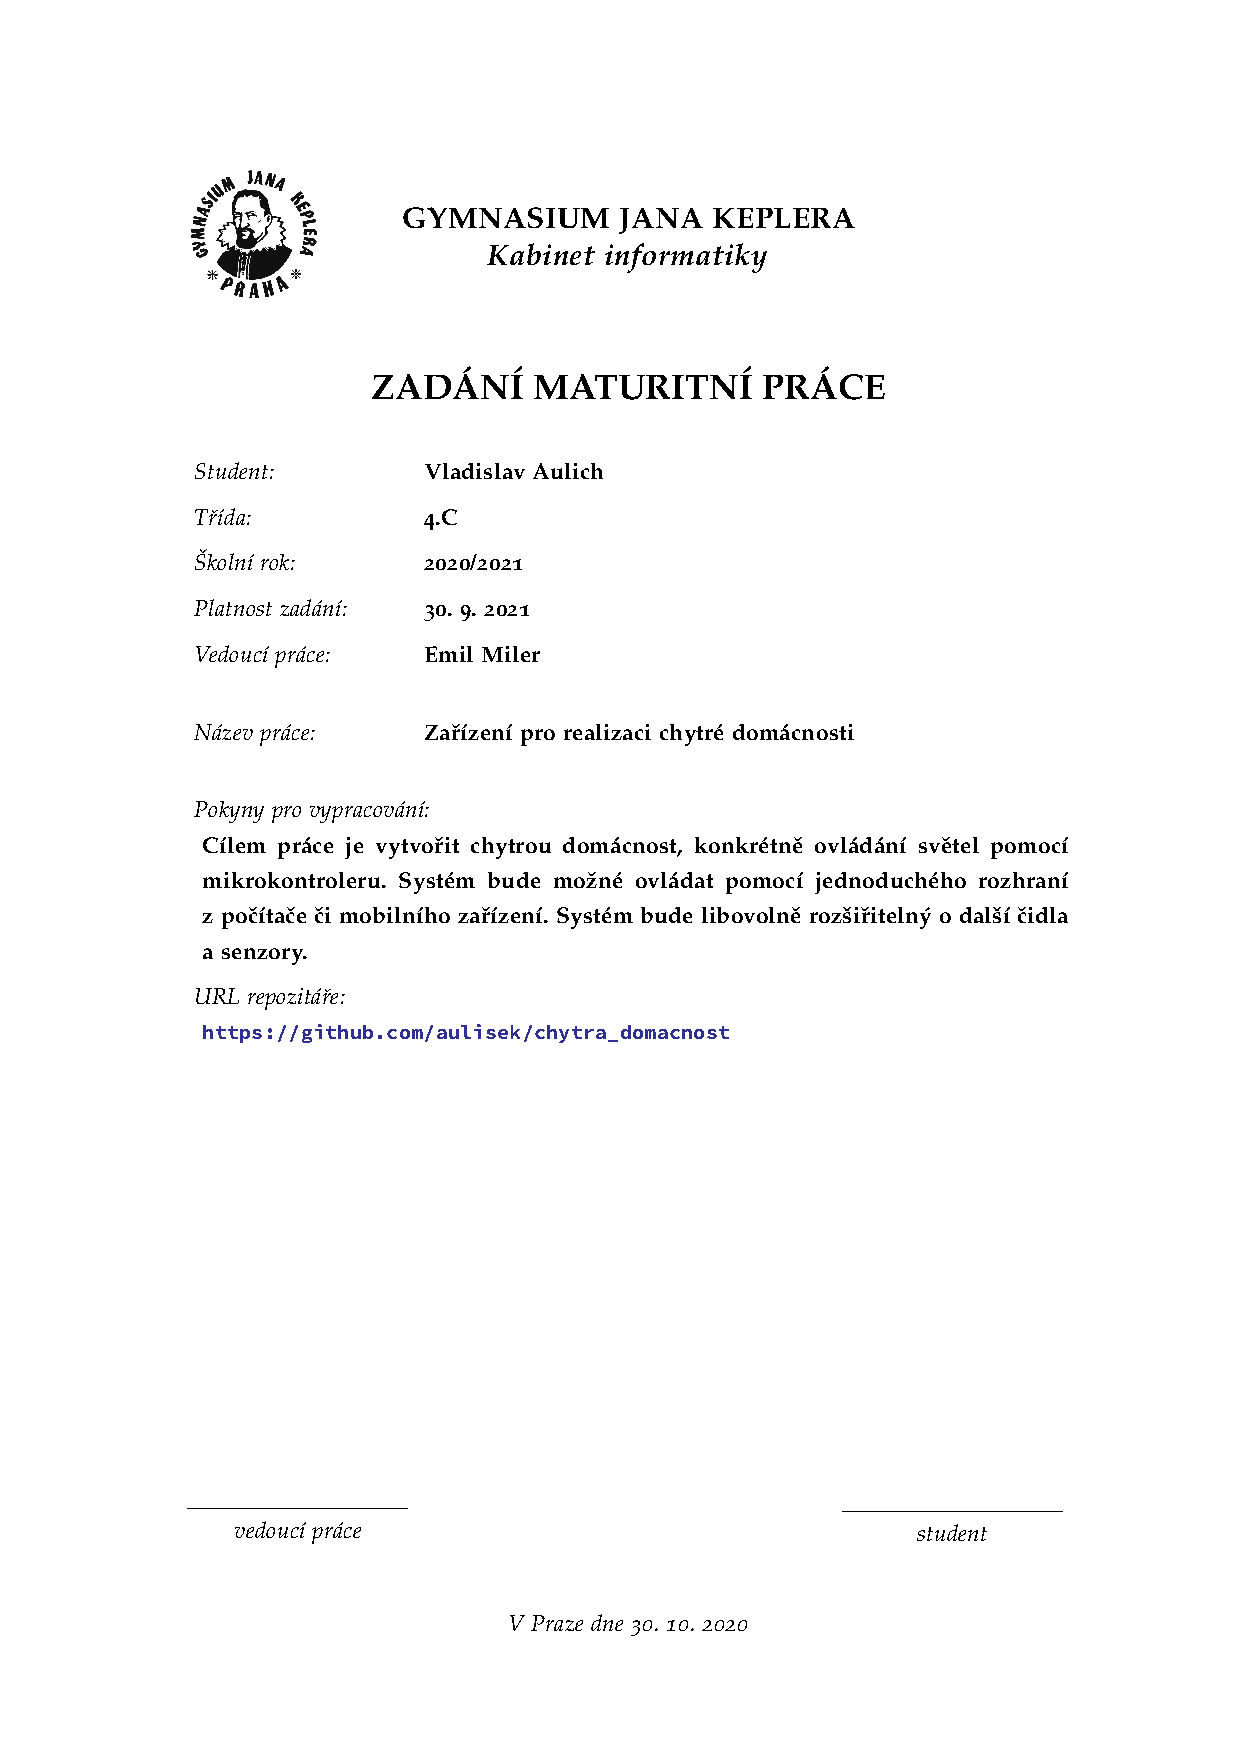
\includepdf[]{zadani.pdf}


%%% Strana s čestným prohlášením k bakalářské práci

\hypersetup{pageanchor=true}
\cleardoublepage
\vspace*{\fill}
\section*{Prohlášení}
\noindent
\Prohlaseni

\vspace{2cm}
\noindent
V Praze dne \today
\hspace*{\fill}\small{\AutorPrace}
\vspace{1cm}

%%% Poděkování
\openright
\vspace*{\fill}
\section*{Poděkování}
\noindent
\Podekovani
\vspace{1cm}


%%% Povinná informační strana bakalářské práce
\openright
\section*{Abstrakt}
\noindent
\Abstrakt
\subsection*{Klíčová slova}
\noindent
\KlicovaSlova

\bigskip\bigskip\bigskip
\section*{Abstract}
\noindent
\AbstraktEN
\subsection*{Keywords}
\noindent
\KlicovaSlovaEN

\openright
\pagenumbering{arabic}

% Obsah
\setcounter{tocdepth}{2}
\tableofcontents

\chapter{Teoretická část}
\pagestyle{fancy}

V první části maturitní práce by se měla objevit informace o tom, jaký problém řešíte. Co si Váš projekt klade za cíl?

\section{Úvod}

Toto téma jsem si zvolil, protože jsem chtěl blíže prozkoumat práci s platformou Arduino a ESP32. S programováním těchto zařízení jsem měl minimální zkušenosti, proto pro mě byla práce na projektu výzvou k objevování nového. Použití komunikace na rádiové frekvenci jsem zvolil z důvodu široké škály použití a velkého množství příkladů. Zároveň jsem měl doma nevyužívaný ovladač pracující s touto frekvencí.



Motivací k výběru tématu \uv{chytré domácnosti} mi bylo její čím dál větší nasazování v domácnostech a snaha vytvořit si ji po svém. Na mnohých komerčních řešeních mi totiž nevyhovoval způsob ovládání, stejně jako velký zásah do soukromí uživatelů.


\section{Cíl práce}

Cílem této práce je vytvořit zařízení pro realizaci chytré domácnosti. Zařízení si klade za cíl ovládat spotřebiče uživatele tzv. \uv{na dálku}. Součástí řešení musí být uživatelské rozhraní, možnost další automatizace a možnost ovládání \uv{offline}.


\chapter{Implementace}

Druhá kapitola obsahuje detailní informace o tom, jak probíhala implementace. Zde se objeví zdůvodnění výběru technologií, řešení problémů, na které jste narazili, informace o použitých knihovnách apod. Pochvalte se, nikdo to za Vás neudělá. Přiznejte chyby, není to ostuda.


\section{Schéma řešení}

Pro dosažení cíle práce jsem projekt rozdělil na dvě nezávislá zařízení:

\begin{itemize}
	\item Centrály - brány ovládající další zařízení
	\item Koncového zařízení ovládajícího spotřebič
\end{itemize}

Pro každé zařízení jsem pak implementoval potřebné funkce. Dále bylo potřeba zajistit jejich vzájemnou komunikaci.

\subsection{Centrála}

Pro \uv{centrálu} jsem  si vybral platformu ESP32 (konkrétně model NODE-MCU32-S\footnote{https://rpishop.cz/iot/2605-waveshare-nodemcu-32s-esp32-wifi-bluetooth-vyvojova-deska.html}) a to hned z několika důvodů. Čip má integrovanou wifi, k dispozici je velké množství dokumentace, hardwaru s příklady a knihovnami. Další výhodou je velká komunita, což může pomoct při řešení problémů. Čip lze také integrovat do prostředí Arduino IDE, což umožňuje snadnější práci při tvorbě kódu.


Při výběru jsem zvažoval i platformu raspberry pi, ale odradila mě přítomnost operačního systému, který je zbytečný pro tak malý projekt a velké pořizovací náklady oproti ESP32.

Centrála zajišťuje několik funkcí:
\begin{itemize}
	\item Komunikace s uživatelem
	\item Komunikace mezi zařízeními
	\item Správa uložených zařízení
\end{itemize}

\subsubsection{Komunikace s uživatelem}

Pro komunikaci s uživatelem je vytvořeno jednoduché webové rozhraní umožňující dynamicky vypsat uložená zařízení a přidat nové. Pro tvorbu webového rozhraní jsem zvolil knihovnu ESPAsyncWebServer\footnote{https://github.com/me-no-dev/ESPAsyncWebServer}. Tato knihovna má dobře zpracovanou dokumentaci a pro nasazení v projektu se hodí svými funkcemi. Samotné připojení čipu k Wi-Fi je realizováno pomocí knihovny WiFi\footnote{https://github.com/arduino-libraries/WiFi}.


První verze kódu měly implementovaný jednoduchý synchronní webserver pomocí knihovny WiFi, obsažené v základní verzi Arduina IDE. Toto řešení nebylo vhodné, protože numožňovalo připojení více uživatelů k rozhraní naráz.


Další implementovanou funkcí byla autentifikace uživatele. Tato funkce je zajištěná při odesílání requstu pomocí knihovny ESPAsyncWebServer.


Pro zjednodušení přístupu k uživatelskému rozhraní je na zařízení spuštěn mDNS server na adrese http://esp32.local. Tato funkce je realizována pomocí knihovny ESPmDNS \footnote{https://github.com/espressif/arduino-esp32/tree/master/libraries/ESPmDNS}.


Uživatelské rozhraní je vytvořeno pomocí HTML. HTML soubor je uložen ve vnitřní flash paměti čipu ESP. K ovládání filesystému SPIF je užito knihovny SPIFFS\footnote{https://github.com/espressif/arduino-esp32/tree/master/libraries/SPIFFS}. Tato knihovna obsahuje všechny potřebné funkce.


Pro přidání nového zařízení má uživatel na výběr mezi přidáním koupeného komerčního zařízení nebo přidáním zařízení vyrobeného v rámci tohoto projektu. Postup při zadávání nového zařízení je nastíněn we webovém rozhraní.


Komunikace programu a webového rozhraní je zajištěna pomocí HTTP GET requestů, které program zpracuje a provede potřebné akce. 


\subsubsection{Komunikace mezi zařízeními}

Komunikace mezi zařízeními je realizovaná bezdrátově po frekvenci 433 MHz. Tento druh jsem zvolil z důvodu rozšířenosti a nízkých pořizovacích nákladů modulů\footnote{https://www.laskarduino.cz/sada-vysilac-prijimac-433mhz/}. Další nespornou výhodou je dosah, který v optimálním prostředí může být až 200 m.


Další ze zvažovaných řešení byla realizace pomocí Wi-Fi nebo GSM modulu. V prvním případě jsem jako nevýhodu viděl dosah (závislost na dostupnosti připojení). Dále by nebylo tak snadné ovládat zařízení pomocí ovladače. V druhém případě byla nevýhoda cena a potřeba realizace připojení pomocí telefoního operátora.


Ovládání modulů jsem chtěl realizovat pomocí jednoduché knihovny VirtualWire, ale zjistil jsem, že není funkční na čipech ESP. K ovládání jsem tak použil knihovnu RadioHead. 


Pro ovládání \uv{Koncového zařízení} je vyslána zpráva obsahující ID zařízení a tag ON nebo OFF, \uv{koncové zařízení} následně odchytí ID a provede příkaz. Tento systém je do budoucna rozšiřitelný o další tagy pro zařízení, které potřebují k ovlání více příkazů než ON nebo OFF.


Tento navržený systém jsem implementoval, nicméně jsem narazil na problém s ovládáním pomocí komerčního ovladače. K tomuto účelu jsem začlenil knihovnu RCswitch\footnote{https://github.com/sui77/rc-switch}, která umožňuje zobrazit protokol, na jehož základě právě komerční zařízení komunikují. Poté dokáže vysílat tímto protokolem. 


Ve svém řešení jsem chtěl použít knihovny obě a rozdělit tak ovládání na dvě části, podle toho, jakým způsobem mají komunikovat. Při realizaci tohoto jsem však narazil na problém, že není možné bezdrátový vysílač ovládat dvěma knihovnami současně.


Nakonec jsem vybral knihovnu RCswitch z důvodu větší spolehlivosti při přenosu vysílání a možného rozšíření na ovládání komerčních zařízení (nebo ovládání komerčními zařízeními). Toto řešení sebou nese nutnost dvou kódů, pro zapnutí a vypnutí (při použití již výše zmiňovaného ovladače). 


\subsubsection{Správa uložených zařízení}

Zařízení se ukládají přímo do flash paměti ESP32 o velikosti 4 MB. Soubor je nazván \uv{zarizeni.csv}. Zařízení se ukládají ve formátu CSV (comma separate value). Pro ovládání filesystému byla zvolena výše zmíněná knihovna SPIFFS. Pro \uv{parsování} csv souboru jsem využil již hotové řešení za pomocí knihovny CSVparser\footnote{https://github.com/michalmonday/CSV-Parser-for-Arduino}. Knihovna je pěkně zadokumentovaná a obsahuje vše, co jsem pro čtení CSV potřeboval. 


Do sloupce \uv{název} se uloží název, který si zadá sám uživatel v uživatelském rozhraní. Do sloupce \uv{kod\_ovladac} se v případě zařízení vyrobeného v rámci projektu uloží \uv{x}, protože k ovládání stačí ID zařízení, které je v tomto případě ve sloupci \uv{kod\_zarizeni}.


Při zadávání komerčního zařízení záleží na způsobu ovládání daného zařízení. Při tvorbě jsem vycházel z mého ovladače, který má zvlášť kód pro vypnutí a zapnutí. Jiná zařízení mají odlišná schémata. 


Pro implementaci takového typu zařízení je za potřebí analyzovat, jaký způsob ovládání zařízení používá. K tomu slouží example kód knihovny RCswitch. Pro funkčnost ovládání je také potřeba prostudovat dokumentaci k této knihovně a dopsat správný typ ovládání do místa v kódu (Toto místo je označeno přímo v kódu).

\subsection{Koncové zařízení}

Toto je hlavní částí mého projektu. Koncové zařízení provádí následující funkce:

\begin{itemize}
	\item přijímá požadavek od centrály
	\item zapne/vypne spotřebič
	\item reaguje na pohyb
	\item obsahuje senzor světla 
	\item reaguje na vstup uživatele z tlačítka
\end{itemize}

Pro \uv{koncová zařízení} jsem zvolil jako vývojovou platformu Arduino uno\footnote{https://www.laskarduino.cz/arduino-uno-r3--atmega328p--klon/}. Po odladění kódu a hardwaru jsem vyrobil prototyp, který již využíval Arduino Pro mini\footnote{https://www.laskarduino.cz/arduino-pro-mini--atmega328-5v-16mhz--klon/} s pšti voltovou logikou. 


Pro realizaci zapínání a vypínání spotřebičů jsem zvolil ovládání pomocí relé. Pro snadnější ovládání jsem vybral již hotový modul pro arduino\footnote{https://dratek.cz/arduino/2954-modul-rele-5v-1-kanal-opticky-oddeleno.html}, který pokud je na vstupu logická 1 vypnutý, pokud je přítomna zem, tak je zapnutý (je tzv. negovaný).


Reakce na pohyb je zajišťována PIR senzorem\footnote{https://www.laskarduino.cz/arduino-pir-detektor-pohybu-hc-sr501/}. Opět byl zakoupen modul, který bylo snazší implementovat. Aby nedocházelo k zapnutí světla ve dne, byl k senzoru přidán fotorezistor, který reaguje na hladinu světla v místnosti. Při tvorbě kódu pro fotorezistor jsem narazil na problém s rozeznáváním světla od tmy. Fototorezistor v mém zapojení totiž neukazoval konstantní hodnoty.


Při prvním pokusu ovládání jsem nastavil pevnou hranici pro tmu, kde jsem porovnával napětí na analogovém vstupu s pevně danou hodnotou. Toto řešení se neukázalo jako vhodné ve chvíli. kdy fotorezistor ukazoval hodnoty blízké k hranici, docházelo tak k rychlému spínání a vypínání světla. Ve finálním kódu jsem použil hystereze a k tomuto efektu nedochází. Nevýhoda tohoto řešení je, že si uživatel musí nastavit hranici tmy v kódu. Toto by se dalo vyřešit náhradou rezistoru za trimmer, kterým by uživatel měnil hodnotu odporu a s tím i napětí na amalogovém vstupu.


Při pátrání na internetu jsem objevil právě takový modul\footnote{https://www.laskarduino.cz/arduino-svetelny-senzor--4-pin-modul/}, který umožňoval trimmerem měnit \uv{citlivost na tmu}. Proto jsem ho zakoupil a ve výsledném řešení je implementován. Samotný modul má dva výstupy. Jeden je analogový ukazující \uv{hladinu tmy} a druhý je digitální, který má buď logickou jedničku na světle, zem při tmě. Toto zapojení se tak i hodí k negovanému relé, kde lze zapojit modul napřímo k ovládání relé bez nutnosti mikrokontroleru.
\begin{figure}[htb]
\centering
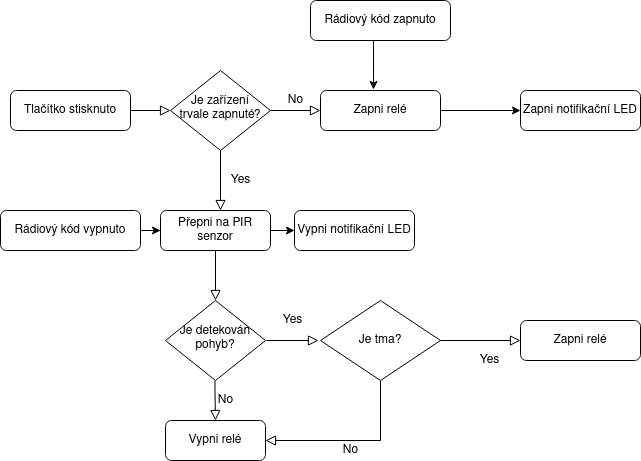
\includegraphics[width=1\hsize]{img/schema_koncove_zarizeni.png}
\caption{Schéma činností koncového zařízení}\end{figure}

\section{Návrh prototypu}
\subsection{Centrála}

Centrálu jsem se rozhodl ponechat v nepájivém kontaktním poli a vyrobit k ní krabičku na 3D tiskárně. Návrh krabičky pro 3D tisk jsem tvořil v programu thinkercad. 

Obrázek Schéma zapojení

\subsection{Koncové zařízení}

\subsubsection{Pokus 1}

Oddělení na snímání pohybu pomocí PIR čidla a ovládání pomocí tlačítka (ovladače) jsem původně chtěl rozdělit hardwarově. Jedna část by bylo Arduino, které přijímá kód po rádiu a vstup uživatele z tlačítka a druhá část by byl PIR senzor, který obstarává vše ostatní.


Protože PIR senzor má vlastní časovač, logickou 1 dává na výstup vždy podle uživatele nadefinovanou dobu od posledního pohybu. Toho jsem chtěl využít a spojit výstup arduina pomocí dvou diod s výstupem PIR senzoru a připojit to na vstup relé. Toto řešení však sebou neslo spoustu nevýhod. 

\begin{figure}[htb]
\centering
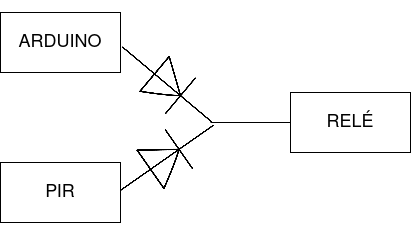
\includegraphics[width=0.5\hsize]{img/zapojeni_rele.png}
\caption{Schéma zapojení relé a diody}\end{figure}

Toto řešení nefungovalo perfektně, kvůli úbytku napětí na diodě (0.7 V), takže výstup s PIR nebyl iniciován jako logická 1. Další nevýhodou byl fakt, že používám negované relé. Tyto problémy by šly vyřešit použitím tranzistoru, nicméně i kvůli detektoru hladiny světla jsem toto řešení zavrhl.

\subsubsection{Pokus 2}

Po prvním nezdařilém pokusu jsem přešel na kompletní ovládání arduinem. Nejprve jsem si všechny potřebné díly spojil v nepájivém kontaktním poli a potom jsem ověřil funkčnost kódu. Takto vyrobené zařízení splňovalo všechny požadavky, takže jsem se rozhodl zařízení přenést do kompaktnější podoby.


\begin{figure}[htb]
\centering
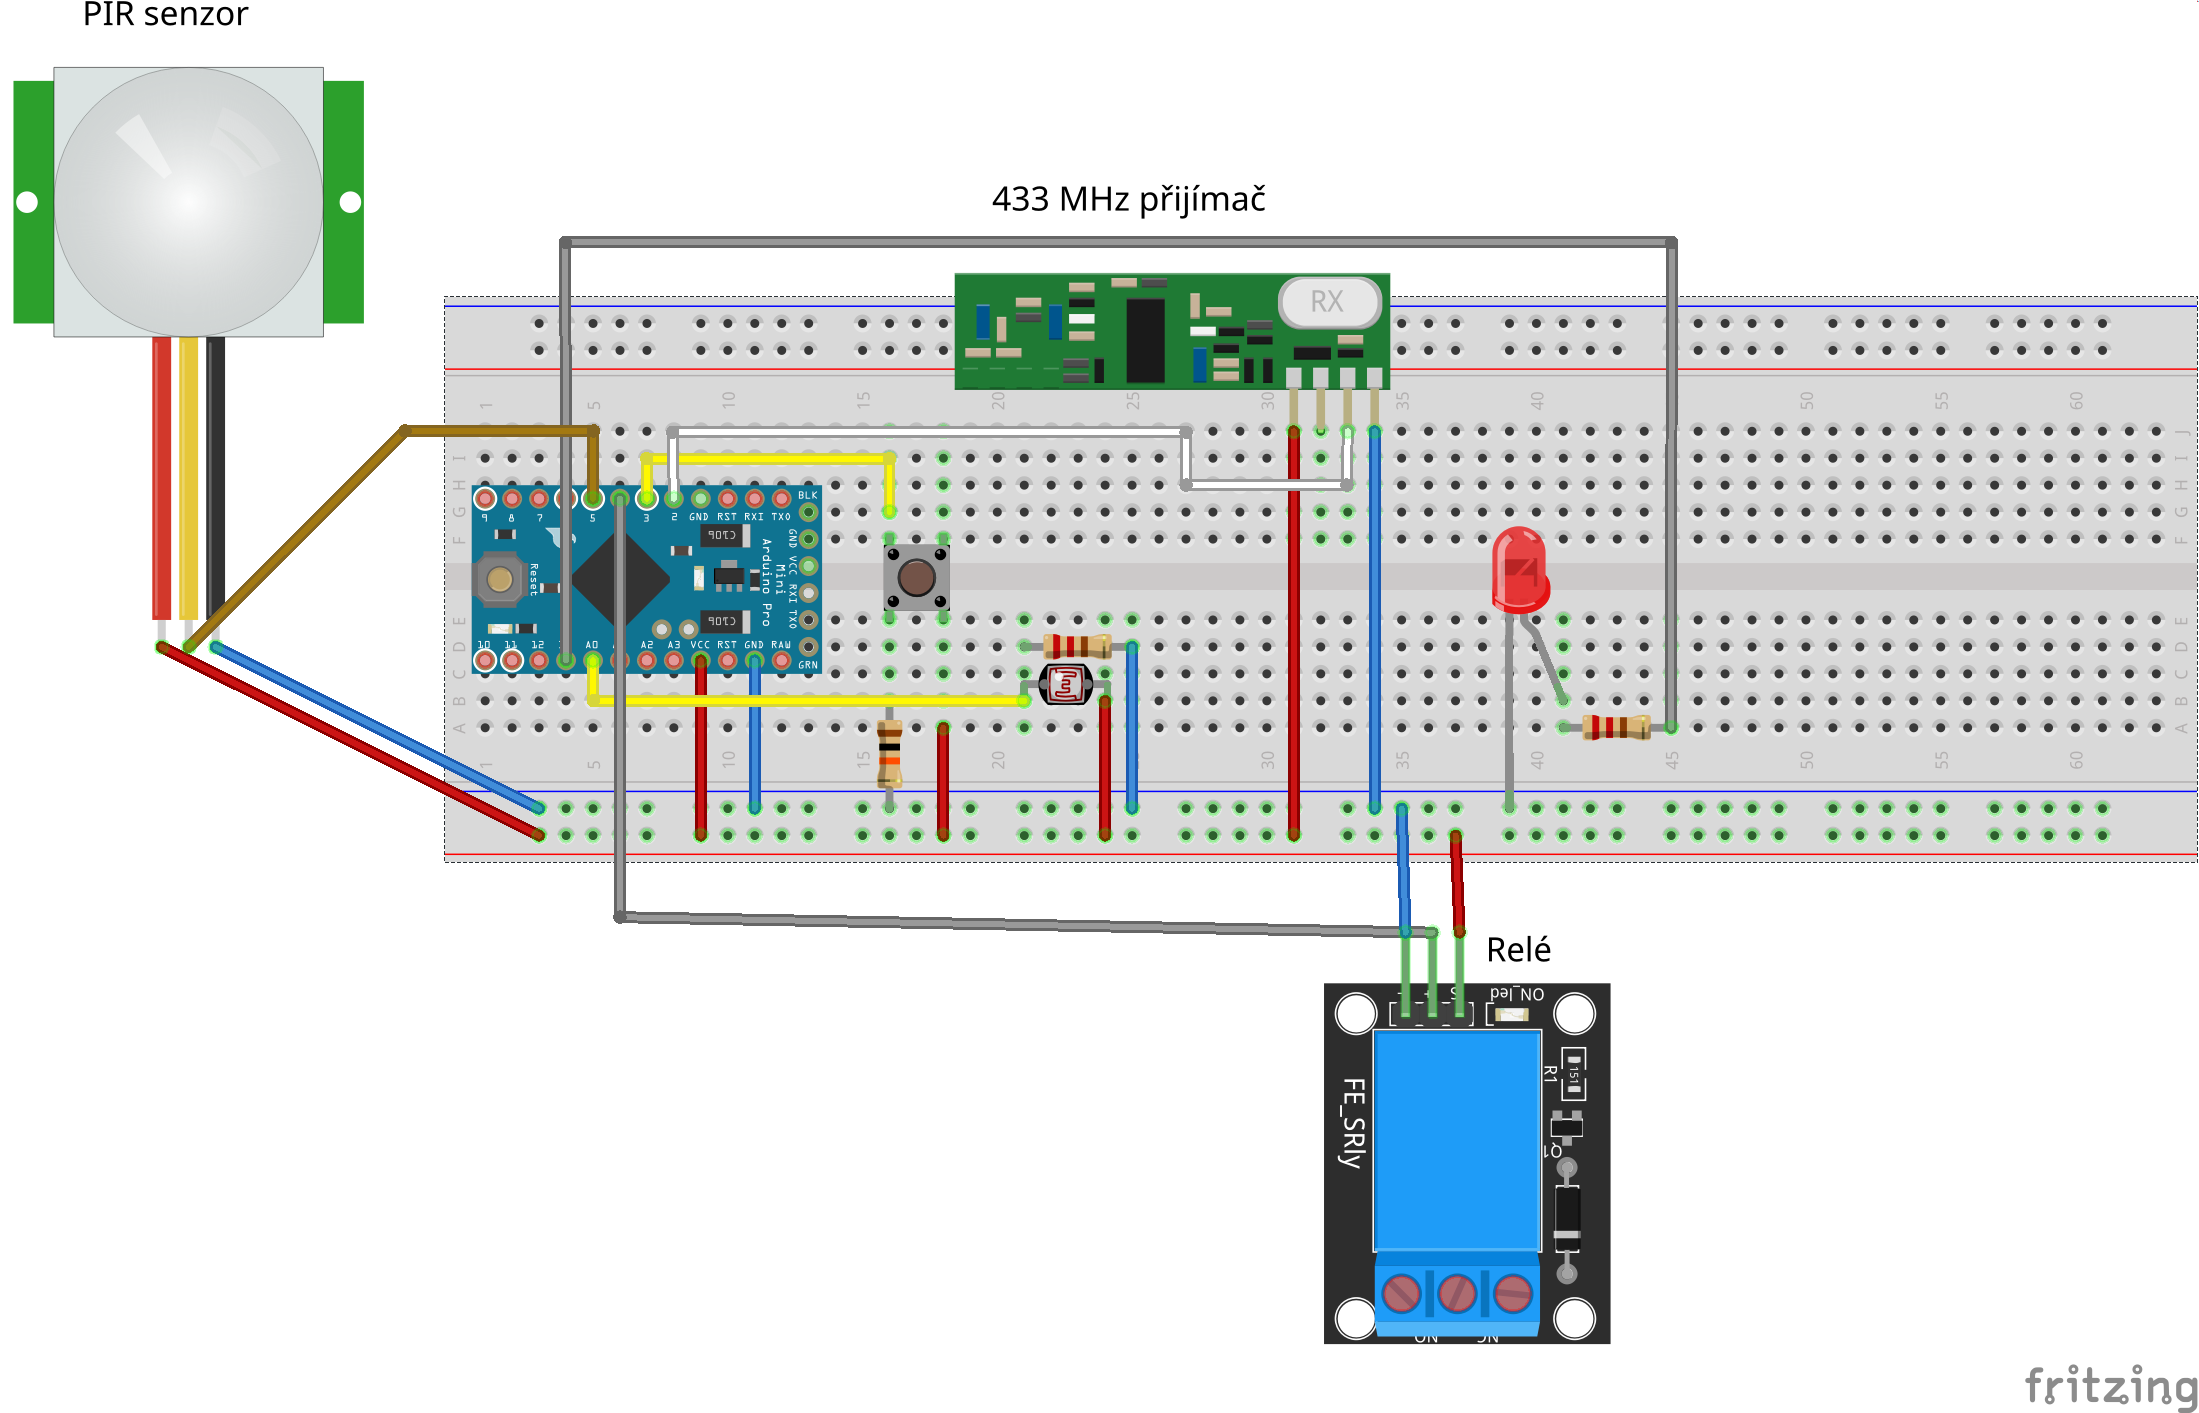
\includegraphics[width=1\hsize]{img/přijímač_zásuvka_bb.png}
\caption{Schéma zapojení v nepájivém kontaktním poli}\end{figure}

Opět jsem vytvořil návrh krabičky pro 3D tisk. Při návrhu krabičky pro PIR senzor jsem vycházel již z hotového modelu\footnote{https://www.thingiverse.com/thing:2845890} staženého z portálu thinkverse, který jsem obohatil o díru na fotorezistor a notifikační LED. Návrh je od autora hills8, publikován je pod licencí creative commons-attribution. Návrh krabičky pro zařízení jsem již vytvářel sám. Moduly jsem následně přenesl na zakoupenou PCB návrhovou desku podle schématu.


\section{Výroba prototypu}

Tisk součástek jsem prováděl na tiskárně Ender 3 pro, kterou jsem si sám složil. Při pájení součástek na desku jsem narážel na nedostatečné vybavení, ale myslím, že jsem nakonec udělal co bylo v mých silách. 

\subsection{3D tisk}


\subsection{Kalkulace nákladů}

\begin{table}[htb]
\centering
\begin{tabular}{|c|c|c|}
	\hline
	Počet kusů & Název & Cena [Kč] \\
	\hline
	1 & NodeMCU-32S ESP32 & 249  \\
	\hline
	2 & 433 MHz vysílač a přijímač & 79 \\
	\hline
	2 & Spirálová anténa 433 MHz & 10 \\
	\hline
	1 & Mikrospínač & 4 \\
	\hline
	2 & Relé modul s optickým oddělením & 65 \\
	\hline
	1 & Rezistor 10k & 1 \\
	\hline
	1 & Arduino Pro Mini & 98 \\
	\hline
	1 & Arduino uno & 599 \\
	\hline
	1 & PCB prototypová deska & 18 \\
	\hline
	1 & PIR detektor pohybu & 38 \\
	\hline
	1 & Detektor tmy & 20 \\
	\hline
\end{tabular}
\caption{Kalkulace nákladů}
\end{table}

Celkové náklady na \uv{centrálu} bez 3D tisku jsou přibližně 300 Kč.
Celkové náklady za prototyp \uv{koncového zařízení} bez 3D tisku je 265 Kč.

\section{Možnosti automatizace}

\section{Návrhy na vylepšení}

\chapter{Technická dokumentace}

Poslední kapitola obsahuje informace o tom, jak projekt, který v rámci maturitní práce vznikl, nainstalovat, spustit a používat.

\section{Ukázka sekce}


\subsection{A jedné podsekce}


\section{A další sekce}


\chapter*{Závěr}
\pagestyle{empty}
\addcontentsline{toc}{chapter}{Závěr}


Závěr obsahuje shrnutí práce a vyjadřuje se k míře splnění jejího zadání. Dále by se zde mělo objevit sebehodnocení studenta a informace o tom, co nového se naučil a jak vnímal svou práci na projektu.

V rámci projektu jsem vytvořil funkční soustavu zařízení umožňující realizaci chytré domácnosti. Toto zařízení splňuje všechny body zadání. Se zařízením jsem spokojený, splňuje všechny mé požadavky. Do budoucna se nabízí rozšíření a vylepšení zařízení.


Při tvorbě projektu jsem si osvojil mnoho nových dovedností. Při sofwarovém návrhu jsem se blíže seznámil s prostředím Arduino IDE, práci s knihovnami a dokumentací. Naučil jsem se práci se senzory a způsoby jejich připojení. Při tvorbě webového prostředí nasazení HTML a kaskádových stylů. K zaznamenávání verzí projektu jsem používal verzovací systém git, změny jsem nahrával na server github. Bylo to moje první setkání s verzovacími systémy, ze začátku jsem trochu tápal, jak ho přesně použít. Při tvorbě kódu jsem však ocenil přehlednost a vracení se ke starším verzím. Systém jsem ovládal z příkazové řádky, naučil jsem se tak spravovat svůj soborový systém a efektivní práci s ním.


Realizace hardwarové části mi přinesla zkušenost s letováním, nahráváním programu do Arduina pro mini pomocí programátoru mimo prostředí Arduino IDE. Také jsem se naučil základy programu fritzing při tvorbě schémat zapojení modulů. Naučil jsem se základy 3D modelování pomocí softwaru thinkercad, následné převedení předlohy modelu do hotové podoby použitím metody 3D tisku. S tím se pojí i samotná údržba 3D tiskárny. Po jejím složení jsem se rozhl pro několik úprav. Seznámil jsem se s firmwarem Marlin, naučil jsem se ho upravovat, zkompilovat a nahrát ho do tiskárny za použití USBisp programátoru. Dále jsem se dozvěděl více o materiálech pro 3D tisk a potřebným nastavením parametrů tisku.


Při tvorbě dokumentace jsem se seznámil se zázecím sytémem \LaTeX, který pro mě byl nový 

%%% Seznam použité literatury
\nocite{einstein}\nocite{maly}\nocite{knuthwebsite}\nocite{ucebnice}\nocite{polovodicovatechnika}\nocite{šrait}\nocite{techtutorials}
\printbibliography[title={Seznam použité literatury},heading={bibintoc}]

%%% Seznam obrázků
\openright
\listoffigures
\addcontentsline{toc}{chapter}{Seznam obrázků}

%%% Seznam tabulek
\clearpage
\listoftables
\addcontentsline{toc}{chapter}{Seznam tabulek}

%%% Přílohy k práci, existují-li. Každá příloha musí být alespoň jednou
%%% odkazována z vlastního textu práce. Přílohy se číslují.

%\part*{Přílohy}
%\appendix

\end{document}
